\paragraph{}
Naša topológia siete pozostáva z firewallu ku ktorému je na jednom rozhraní pripojený prepínač ku ktorému su napojené dva servery a dva počítače. Na druhom rozhraní je Internet. Na linuxoch aj na windowsoch bola rovnaká topológia s výnimkou, že pri pracovaní s linuxom sa nachádzali počítače a servery v rozdielnych VLAN: Servery vo VLAN-e 10 a desktopy vo VLAN-e 20.
\paragraph{}
Keďže si Windows Server nerozumel s VLAN-ami, topológia siete sa líši v tom, že všetky koncové uzly sú v defaultnej VLAN-e (VLAN 1).

\begin{figure}[h]
\centering
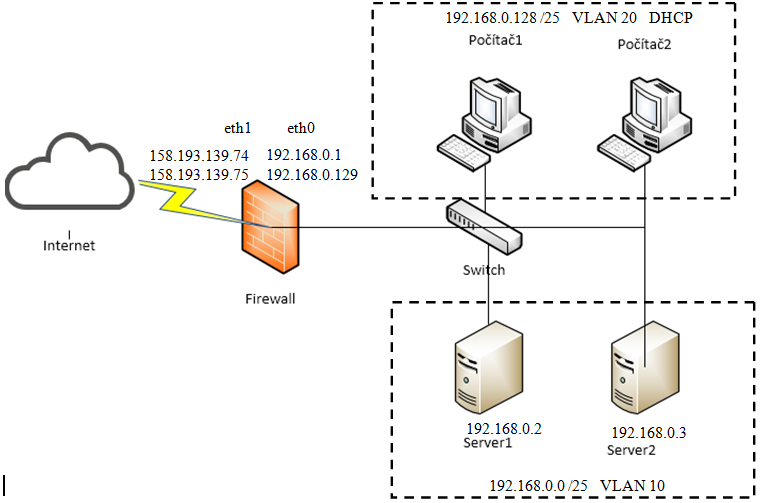
\includegraphics[scale=0.5]{general_logicka_topologia}
\caption{Logická topológia siete}
\label{fig:log_topologia}
\end{figure}
